%------------------------------------------------------------------------------
% Este é um template para documentação textual de um projeto Java. 
%
%------------------------------------------------------------------------------


%------------------------------------------------------------------------------
% Modelo livro de documento. Configurado para papel a4 e fonte de 12 pontos e
% openany evita que seja gerada uma página em branco logo após o índice.
%------------------------------------------------------------------------------
\documentclass[a4paper,12pt,openany]{book}
%------------------------------------------------------------------------------
%  Utiliza idioma Português do Brasil e codificação utf8 para exibir caracteres
%  acentuados.
%------------------------------------------------------------------------------
\usepackage[brazilian]{babel}
\usepackage[utf8]{inputenc}
%------------------------------------------------------------------------------
%  Pacote gráfico para incluir figuras no documento.
%------------------------------------------------------------------------------
\usepackage{graphicx}
%-----------------------------------------------------------------------------
% Pacote para criar minipages: caixas de texto com fundo colorido.
%-----------------------------------------------------------------------------
\usepackage[svgnames]{xcolor} 
%-----------------------------------------------------------------------------
% Define cores de fundo para minipages.
%-----------------------------------------------------------------------------
\definecolor{lightblue}{RGB}{173,216,230} 
\definecolor{lightgrey}{RGB}{211,211,211}
%-----------------------------------------------------------------------------
% Define as margens do documento.
%-----------------------------------------------------------------------------
\usepackage{geometry}
\geometry{left=1cm,right=1cm,top=5cm,bottom=2cm}


\begin{document}

\author{Versão 1.0}
\title{Huugle}
\date{\today}


\maketitle

%------------------------------------------------------------------------------
%  Cria um índice do documento nomeado como Índice
%------------------------------------------------------------------------------
\renewcommand{\contentsname}{Índice}
\tableofcontents

\newpage

%------------------------------------------------------------------------------
% Capítulo introdutório da documentação
%------------------------------------------------------------------------------
\chapter*{Desenvolver Simples Ferramenta de Pesquisa para o Acervo do Clube Cético}
\addcontentsline{toc}{chapter}{Desenvolver Simples Ferramenta de Pesquisa para o Acervo do Clube Cético}

O objetivo deste projeto é desenvolver em Java um motor de busca para localizar tópicos 
e postagens de interesse a partir de palavras chave.
\\\\
O programa deve ter uma interface que permita digitar até 5 palavras chave, selecionar ou 
não um nickname de forista para restringir a pesquisa, selecionar ou não um intervalo 
entre datas para restringir a pesquisa, selecionar se a pesquisa deverá ser realizada
em textos de postagens ou em títulos de tópicos, e se os resultados apresentados serão
na forma de links para páginas do acervo armazenadas localmente ou para páginas hospedadas 
online no servidor.
\\\\
A Fig. \ref{figura:JanelaPrincipal} é uma imagem da janela principal de um protótipo do programa.

\begin{figure}[h]
	\centering % para centralizarmos a figura
	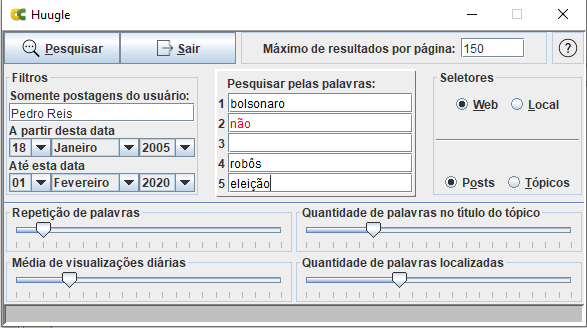
\includegraphics[width=15cm]{Figuras/principal.png} % leia abaixo
	\caption{Janela Principal}
	\label{figura:JanelaPrincipal}
\end{figure}

A função dos controles deslizantes mostrados na figura serão especificadas mais adiante.
\\\\
As classes a serem desenvolvidas estarão distribuídas pelos seguintes pacotes:
\begin{description}
	\item[br.com.hkp.searchengine.buildfiles] Classes para construir os arquivos da base de dados do programa
	\item[br.com.hkp.searchengine.json] Classes que implementam a leitura de arquivos json de serão extraídos os dados
	\item[br.com.hkp.searchengine.register] Classes que implementarão os registros dos arquivos na base de dados. E devem prover a funcionalidade para ler e gravar tais arquivos. 
	\item[br.com.hkp.searchengine.gui] O pacote que implementa a interface gráfica
	\item[br.com.hkp.searchengine.util] Pacote que deve prover métodos de uso geral e definições de variáveis e constantes globais.
	\item[br.com.hkp.searchengine.main] Pacote do programa principal. 
\end{description}

Vamos iniciar o desenvolvimento da nossa aplicação pelo pacote \textit{register.}...




\newpage

%*****************************************************************************
% As próximas seções "part" documentam, cada uma, um dos pacotes que constituem
% o projeto.
%*****************************************************************************
 
%------------------------------------------------------------------------------
% Cada seção "part" deste documento deve ser referente a um pacote do projeto.
%
% O texto no início de cada seção "part" aborda e elucida a função do pacote no
% projeto a que ele pertence.
%------------------------------------------------------------------------------
\colorbox{lightblue}{
	
\begin{minipage}{18cm}
	
\part*{register}
\addcontentsline{toc}{part}{br.com.hkp.searchengine.register}

\paragraph{br.com.hkp.searchengine.register}

As pesquisas não serão realizadas sobre os arquivos HTML do acervo, mas em uma base de 
dados composta por uma coleção de arquivos de acesso aleatório de objetos.\\
\\
A maioria destes arquivos deve estar ordenada por uma chave primária para permitir 
pesquisa binária, e cada classe desse pacote deve ser a definição do registro de um destes arquivos, além de prover o todo o código necessário para leitura, gravação, pesquisa binária e demais operações necessárias sobre estes arquivos.\\
\\
A primeira classe a ser construída é Register, que deve ser a superclasse das demais classes neste pacote. Provendo métodos e definições comuns às subclasses.\\
\\



\end{minipage}

}%fim da caixa de texto com fundo colorido

\newpage

%*****************************************************************************
% As próximas seções "chapter" documentam, cada uma, uma das classes que
% constituem o pacote documentado nesta seção "part".
%*****************************************************************************

%------------------------------------------------------------------------------
% Documenta a primeira classe do pacote. 
%------------------------------------------------------------------------------
\colorbox{lightgrey}{
	
\begin{minipage}{18cm}
	
\chapter*{Register}
\addcontentsline{toc}{chapter}{Register}

\paragraph{Register}

PONHA AQUI o texto documentando a classe

\end{minipage}

}%fim da caixa de texto com fundo colorido

\newpage

%*****************************************************************************
% As próximas seções "section" documentam, cada uma, um dos métodos que
% constituem a classe documetada  nesta seção "chapter".
%*****************************************************************************

%------------------------------------------------------------------------------
% Documenta primeiro método da classe a qual é referente esta seção "chapter".
%------------------------------------------------------------------------------
\section*{PONHA AQUI o Cabeçalho do Método}
\addcontentsline{toc}{section}{PONHA AQUI o Nome do Método}

\newpage

%------------------------------------------------------------------------------
% A partir dessa tag todos os capítulos são interpertados pelo Latex como 
% apêndices e indexados por letras em vez de números.
%------------------------------------------------------------------------------
\appendix


\chapter{PONHA AQUI o Título do Apêndice}

PONHA AQUI o texto do apêndice.

\newpage



\end{document}